\documentclass{beamer}

\usepackage{graphicx}
\usepackage[normalem]{ulem}
\usepackage{tikz}

\definecolor{arrowcolor}{rgb}{0.5,0.5,1}

\title{Git: Rebase Your Expectations}
\subtitle{How Distributed Version Control Can Save Your Life}
\author{Josh Larson}
\beamertemplatenavigationsymbolsempty

\begin{document}

\newcommand{\commit}[3]{
  \node[circle, draw, radius=0.5cm, fill=green](#1) at #2{\Huge \texttt{#3}};
}
\newcommand{\selectedcommit}[3]{
  \node[circle, draw, radius=0.5cm, fill=cyan, very thick](#1) at #2{\Huge \texttt{#3}};
}
\newcommand{\anoncommit}[2]{
  \node[circle, draw, minimum size=1cm, fill=green](#1) at #2{};
}
\newcommand{\selectedanoncommit}[2]{
  \node[circle, draw, minimum size=1cm, fill=green, thick](#1) at #2{};
}
\newcommand{\branch}[3]{
  \node[draw, fill=yellow](#1) at #2{\texttt{#3}};
}
\newcommand{\selectedbranch}[3]{
  \node[draw, fill=yellow, thick](#1) at #2{\texttt{#3}};
}
\newcommand{\textbox}[3]{
  \node(#1)[draw, fill=white, rounded corners, align=left] at #2 {#3};
}
\newcommand{\squiggle}{\~{}}

\titlepage

\begin{frame}
  \newcommand{\photosize}{0.6\textwidth}

  \frametitle{Photo Syncing}

  \begin{columns}
    \begin{column}{0.35\textwidth}
      \begin{center}
        \textbf{Server}
        \begin{figure}[l]  
          \uncover<1-6,8->{\includegraphics[width=\photosize]{merchmart}}

          \includegraphics[width=\photosize]{shell}

          \uncover<4->{\includegraphics[width=\photosize]{skyline}}
        \end{figure}
      \end{center}
    \end{column}

    \begin{column}{0.3\textwidth}
      \begin{center}
        \uncover<2->{
          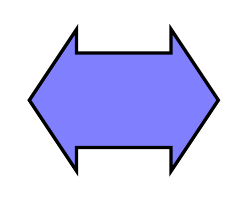
\begin{tikzpicture}[scale=0.3, fill=arrowcolor, draw=black, very thick]
            \filldraw
            (-2,2) --
            (2,2) --
            (2,3) --
            (4,0) --
            (2,-3) --
            (2,-2) --
            (-2,-2) --
            (-2,-3) --
            (-4,0) --
            (-2,3) --
            cycle;
          \end{tikzpicture}
        }
      \end{center}
    \end{column}
    
    \begin{column}{0.35\textwidth}
      \begin{center}
        \textbf{Laptop}
        \begin{figure}
          \uncover<3-5,9->{\includegraphics[width=\photosize]{merchmart}}

          \uncover<3->{\includegraphics[width=\photosize]{shell}}

          \uncover<5->{\includegraphics[width=\photosize]{skyline}}
        \end{figure}
      \end{center}
    \end{column}
  \end{columns}
\end{frame}

\begin{frame}
  \newcommand{\photosize}{0.5\textwidth}

  \frametitle{Photo Versions}

  \begin{columns}
    \begin{column}{0.5\textwidth}
      \begin{itemize}
      \item Changes
        \begin{itemize}
        \item<3-> Add \texttt{merchmart} and \texttt{shell}
        \item<5-> Add \texttt{skyline}
        \item<7-> Remove \texttt{merchmart}
        \end{itemize}
      \end{itemize}
    \end{column}

    \begin{column}{0.5\textwidth}
      \begin{center}
        \uncover<4-7>{\includegraphics[width=\photosize]{merchmart}}
        
        \uncover<4-8>{\includegraphics[width=\photosize]{shell}}
        
        \uncover<6->{\includegraphics[width=\photosize]{skyline}}
      \end{center}
    \end{column}
  \end{columns}
\end{frame}

\begin{frame}
  \newcommand{\photosize}{0.4\textwidth}

  \frametitle<1-10>{Photo Versions}

  \begin{columns}
    \begin{column}{0.5\textwidth}
      \textbf{Server}
      \only<1-5>{
        \uncover<2->{
          \begin{itemize}
          \item Add 2 images
          \item<3-> Add \texttt{merchmart}
          \end{itemize}
        }
      }
      \only<6->{
        \uncover<7->{
          \begin{itemize}
          \item Add 3 images
          \item<9-> \alert<9>{Remove \texttt{merchmart}}
          \end{itemize}
        }
      }
      \begin{center}
        \uncover<1-9>{\includegraphics[width=\photosize]{merchmart}}
        
        \uncover<1->{\includegraphics[width=\photosize]{shell}}
        
        \uncover<1->{\includegraphics[width=\photosize]{skyline}}
      \end{center}
    \end{column}

    \begin{column}{0.5\textwidth}
      \textbf{Laptop}
      \only<1-5>{
        \uncover<2->{
          \begin{itemize}
          \item Add 2 images
          \item<4-> \alert<4>{Add \texttt{merchmart}}
          \end{itemize}
        }
      }
      \only<6->{
        \uncover<7->{
          \begin{itemize}
          \item Add 3 images
          \item<8-> Remove \texttt{merchmart}
          \end{itemize}
        }
      }
      \begin{center}
        \uncover<5>{\includegraphics[width=\photosize]{merchmart}}
        
        \uncover<1->{\includegraphics[width=\photosize]{shell}}
        
        \uncover<1->{\includegraphics[width=\photosize]{skyline}}
      \end{center}
    \end{column}
  \end{columns}
\end{frame}

\begin{frame}
  \begin{center}
    {\Huge Commits}
  \end{center}
\end{frame}

\begin{frame}
  \frametitle{What is a Commit?}

  \begin{itemize}
    \pause
  \item ``Apply \textbf{these changes} to \textbf{this universe} (and some \textbf{other stuff})''
    \begin{itemize}
      \pause
    \item \textbf{``these changes''}: The diff
      \pause
    \item \textbf{``this universe''}: Parent commit
      \pause
    \item \textbf{``other stuff''}: Metadata, like author, timestamp, and commit message
    \end{itemize}
    \pause
  \item \texttt{a8808ba20c1d3d3f26f685d71a29de3e452d82711}
    \pause
  \item \texttt{a8808ba}
  \end{itemize}
\end{frame}

\begin{frame}
  \begin{center}
    {\Huge History?}
  \end{center}
\end{frame}

\begin{frame}
  \begin{center}
    {\Huge Intent}
  \end{center}
\end{frame}

\begin{frame}
  \begin{center}
    {\Huge Ancestry}
  \end{center}
\end{frame}

\begin{frame}
  \frametitle{Ancestry}
  \begin{center}
    \begin{tikzpicture}
      \commit{commit1}{(-5, 0)}{A}
      \commit{commit2}{(-1, 0)}{B}
      \draw (commit1) -- (commit2);

      \uncover<2->{
        \draw [->] (-1.5, -1) -- (1.5, -1)
        node[pos=0.5, below]{Time};
      }
      
      \uncover<4-> {
        \commit{commit3}{(-3, 3)}{D}
        \draw (commit1) -- (commit3);
      }

      \uncover<3-> {
        \commit{commit4}{(3, 0)}{C}
        \draw (commit2) -- (commit4);
      }

      \uncover<5-> {
        \commit{commit5}{(5, 3)}{E}
        \draw (commit4) -- (commit5);
        \draw (commit3) -- (commit5);
      }
    \end{tikzpicture}
  \end{center}
\end{frame}

\begin{frame}
  \frametitle{Merging}

  \begin{center}
    \begin{tikzpicture}
      \anoncommit{commit1}{(-3, 0)}
      
      \anoncommit{foocommit1}{(-1, 0)}
      \draw (commit1) -- (foocommit1);
      \anoncommit{foocommit2}{(1, 0)}
      \draw (foocommit1) -- (foocommit2);

      \uncover<1-8, 15-> {
        \anoncommit{barcommit1}{(-2, 1.5)}
        \draw (commit1) -- (barcommit1);
        \anoncommit{barcommit2}{(-1, 3)}
        \draw (barcommit1) -- (barcommit2);
      }

      \uncover<6-9> {
        \anoncommit{rebasebarcommit1}{(2, 1.5)}
        \draw (foocommit2) -- (rebasebarcommit1);
      }
      \uncover<7-9> {
        \anoncommit{rebasebarcommit2}{(3, 3)}
        \draw (rebasebarcommit1) -- (rebasebarcommit2);
      }
      
      \uncover<3> {
        \anoncommit{mergecommit}{(3, 3)}
        \draw (foocommit2) -- (mergecommit);
        \draw (barcommit2) -- (mergecommit);
      }

      \uncover<1-2, 4-7, 15-> {
        \branch{bar}{(-1, 4)}{bar}
        \draw (bar) -- (barcommit2);
      }
      \uncover<3> {
        \branch{bar}{(3, 4)}{bar}
        \draw (bar) -- (mergecommit);
      }
      \uncover<8-9> {
        \branch{bar}{(3, 4)}{bar}
        \draw (bar) -- (rebasebarcommit2);
      }
      \uncover<10-11> {
        \branch{bar}{(-3, 1)}{bar}
        \draw (bar) -- (commit1);
      }
      \uncover<12-14> {
        \branch{bar}{(1, 1.75)}{bar}
        \draw (bar) -- (foocommit2);
      }
      \branch{foo}{(1, 1)}{foo}
      \draw (foo) -- (foocommit2);

      \uncover<2, 11>{\textbox{}{(0, 5)}{\texttt{git merge foo}}}
      \uncover<5-7, 13>{\textbox{}{(0, 5)}{\texttt{git rebase foo}}}
      \uncover<14, 16->{\textbox{}{(0, 5)}{\texttt{git merge --ff-only foo}}}
      \uncover<17>{
        \draw[very thick, red] (-2.5, 4.5) -- (2.5, 5.5);
        \draw[very thick, red] (2.5, 4.5) -- (-2.5, 5.5);
      }
    \end{tikzpicture}
  \end{center}
\end{frame}

\begin{frame}
  \frametitle{Merge Strategy}

  \begin{center}
    \begin{tikzpicture}
      \anoncommit{commit1}{(-5, 0)}

      \uncover<2-> {
        \commit{commit2}{(-2.5, 0)}{A}
        \draw (commit1) -- (commit2);
        
        \commit{commit3}{(0, 0)}{B}
        \draw (commit2) -- (commit3);

        \uncover<2-3>{
          \branch{foo}{(0, 1)}{foo}
          \draw (foo) -- (commit3);
        }
      }
              
      \uncover<3-> {
        \commit{commit4}{(-3.75, 2)}{C}
        \draw (commit1) -- (commit4);
        
        \commit{commit5}{(-1.25, 2)}{D}
        \draw (commit4) -- (commit5);

        \uncover<3-4>{
          \branch{bar}{(-1.25, 3)}{bar}
          \draw (bar) -- (commit5);
        }
      }

      \uncover<5-> {
        \anoncommit{commit6}{(1.25, 2)}
        \draw (commit5) -- (commit6);
        \draw (commit3) -- (commit6);
      }
        
      \uncover<5> {
        \branch{bar}{(1.25, 3)}{bar}
        \draw (bar) -- (commit6);
      }

      \uncover<6-> {
        \anoncommit{commit7}{(2.5, 0)}
        \draw (commit6) -- (commit7);
        \draw (commit3) -- (commit7);
        
        \branch{master}{(2.5, 1)}{master}
        \draw (master) -- (commit7);
      }

      \uncover<1-3>{
        \branch{master}{(-5, 1)}{master}
        \draw (master) -- (commit1);
      }
      
      \uncover<4-5>{
        \branch{master}{(0, 1)}{master}
        \draw (master) -- (commit3);
      }

      
    \end{tikzpicture}
  \end{center}
\end{frame}

\begin{frame}
  \frametitle{Merge Strategy (Rebase)}

  \begin{center}
    \begin{tikzpicture}
      \anoncommit{commit1}{(-5, 0)}
      
      \commit{commit2}{(-2.5, 0)}{A}
      \draw (commit1) -- (commit2);
      
      \commit{commit3}{(0, 0)}{B}
      \draw (commit2) -- (commit3);

      \uncover<1> {
        \branch{foo}{(0, 1)}{foo}
        \draw (foo) -- (commit3);
      }

      \uncover<1-2> {
        \commit{commit4}{(-3.75, 2)}{C}
        \draw (commit1) -- (commit4);

        \commit{commit5}{(-1.25, 2)}{D}
        \draw (commit4) -- (commit5);
      }

      \uncover<3-4> {
        \commit{commit4_1}{(1.25, 2)}{C}
        \draw (commit3) -- (commit4_1);

        \commit{commit5_1}{(3.75, 2)}{D}
        \draw (commit4_1) -- (commit5_1);
      }

      \uncover<5-> {
        \commit{commit4_2}{(2.5, 0)}{C}
        \draw (commit3) -- (commit4_2);

        \commit{commit5_2}{(5, 0)}{D}
        \draw (commit4_2) -- (commit5_2);
      }

      \uncover<1> {
        \branch{master}{(-5, 1)}{master}
        \draw (master) -- (commit1);
      }
      \uncover<2-5> {
        \branch{master}{(0, 1)}{master}
        \draw (master) -- (commit3);
      }
      \uncover<6-> {
        \branch{master}{(5, 1)}{master}
        \draw (master) -- (commit5_2);
      }

      \uncover<1-2> {
        \branch{bar}{(-1.25, 3)}{bar}
        \draw (bar) -- (commit5);
      }
      \uncover<3-4> {
        \branch{bar}{(3.75, 3)}{bar}
        \draw (bar) -- (commit5_1);
      }
      \uncover<5> {
        \branch{bar}{(5, 1)}{bar}
        \draw (bar) -- (commit5_2);
      }
    \end{tikzpicture}
  \end{center}
\end{frame}

\begin{frame}
  \frametitle{Merge Strategies}
  \begin{center}
    \begin{tikzpicture}
      \anoncommit{commit1}{(-5, 0)}
      
      \commit{commit2}{(-2.5, 0)}{A}
      \draw (commit1) -- (commit2);
      
      \commit{commit3}{(0, 0)}{B}
      \draw (commit2) -- (commit3);

      \commit{commit4_2}{(2.5, 0)}{C}
      \draw (commit3) -- (commit4_2);

      \commit{commit5_2}{(5, 0)}{D}
      \draw (commit4_2) -- (commit5_2);
      
      \branch{master}{(5, 1)}{master}
      \draw (master) -- (commit5_2);
    \end{tikzpicture}
  \end{center}

  \vspace{0.1\textheight}

  \begin{center}
    \begin{tikzpicture}
      \anoncommit{commit1}{(-5, 0)}

      \commit{commit2}{(-2.5, 0)}{A}
      \draw (commit1) -- (commit2);
      
      \commit{commit3}{(0, 0)}{B}
      \draw (commit2) -- (commit3);

      \commit{commit4}{(-3.75, 2)}{C}
      \draw (commit1) -- (commit4);
      
      \commit{commit5}{(-1.25, 2)}{D}
      \draw (commit4) -- (commit5);

      \anoncommit{commit6}{(1.25, 2)}
      \draw (commit5) -- (commit6);
      \draw (commit3) -- (commit6);
              
      \anoncommit{commit7}{(2.5, 0)}
      \draw (commit6) -- (commit7);
      \draw (commit3) -- (commit7);
      
      \branch{master}{(2.5, 1)}{master}
      \draw (master) -- (commit7);
    \end{tikzpicture}
  \end{center}
\end{frame}

\begin{frame}
  \begin{center}
    {\Huge Rewriting History}
  \end{center}
\end{frame}

\begin{frame}
  \begin{center}
    \begin{tikzpicture}
      \commit{commitA}{(-4.5, 0)}{A}
      
      \uncover<1-3, 5-9, 14-16, 18-19> {
        \commit{commitB_1}{(-1.5, 0)}{B}
        \draw (commitA) -- (commitB_1);
      }
      
      \uncover<1-3, 6-9, 14-16, 21-> {
        \commit{commitC_1}{(1.5, 0)}{C}
        \draw (commitB_1) -- (commitC_1);
      }
      
      \uncover<1-3, 7-9, 13-16> {
        \commit{commitD_1}{(4.5, 0)}{D}
        \draw (commitC_1) -- (commitD_1);
      }
      
      \uncover<11-13> {
        \commit{commitC_2}{(-1.5, 0)}{C}
        \draw (commitA) -- (commitC_2);
      }
      
      \uncover<12-13> {
        \commit{commitB_2}{(1.5, 0)}{B}
        \draw (commitC_2) -- (commitB_2);
      }
      
      \uncover<19> {
        \commit{commitD_2}{(1.5, 0)}{D}
        \draw (commitB_1) -- (commitD_2);
      }
      
      \uncover<20-> {
        \commit{commitE_1}{(-1.5, 0)}{E}
        \draw (commitA) -- (commitE_1);
      }
      
      \uncover<2>{\textbox{}{(0, 3)}{\texttt{git rebase -i A}}}
      \uncover<3-6, 8, 14>{
        \textbox{}{(0, 3)}{
          \color<5-6>{white}{\texttt{pick B}}\\
          \color<6>{white}{\texttt{pick C}}\\
          \texttt{pick D}
        }
      }

      \uncover<9-12>{
        \textbox{}{(0, 3)}{
          \color<11->{white}{\texttt{pick C}}\\
          \color<12->{white}{\texttt{pick B}}\\
          \texttt{pick D}
        }
      }

      \uncover<15>{
        \textbox{}{(0, 3)}{
          \texttt{pick B}\\
          \texttt{pick D}\\
          \texttt{pick C}
        }
      }

      \uncover<16-20>{
        \textbox{}{(0, 3)}{
          \color<18->{white}{\texttt{pick B}}\\
          \color<20->{white}{\texttt{fixup}} \color<19->{white}{\texttt{D}}\\
          \texttt{pick C}
        }
      }
    \end{tikzpicture}
  \end{center}
\end{frame}

\begin{frame}
  \begin{center}
    {\Huge Pitfalls}
  \end{center}
\end{frame}

\begin{frame}
  \begin{center}
    {\Huge Remotes}
  \end{center}
\end{frame}

\begin{frame}
  \begin{center}
    \begin{tikzpicture}
      \anoncommit{remotecommit1}{(-4, 1.5)}
      \anoncommit{remotecommit2}{(-2, 1.5)}
      \draw (remotecommit1) -- (remotecommit2);
      
      \uncover<6->{
        \anoncommit{remotecommit3}{(0, 1.5)}
        \draw (remotecommit2) -- (remotecommit3);
      }

      \uncover<1-5>{
        \branch{remotemaster}{(-2, 2.5)}{master}
        \draw (remotemaster) -- (remotecommit2);
      }
      \uncover<6->{
        \branch{remotemaster}{(0, 2.5)}{master}
        \draw (remotemaster) -- (remotecommit3);
      }

      \draw[dotted] (-5, 0) -- (5, 0);

      \uncover<3->{
        \anoncommit{localcommit1}{(-4, -1.5)}
        \anoncommit{localcommit2}{(-2, -1.5)}
        \draw (localcommit1) -- (localcommit2);
      }
      \uncover<8->{
        \anoncommit{localcommit3}{(0, -1.5)}
        \draw (localcommit2) -- (localcommit3);
      }
      
      \uncover<4-7>{
        \branch{originmaster}{(-2, -2.5)}{origin/master}
        \draw (originmaster) -- (localcommit2);
      }
      \uncover<8->{
        \branch{originmaster}{(0, -2.5)}{origin/master}
        \draw (originmaster) -- (localcommit3);
      }

      \uncover<5-10>{
        \branch{localmaster}{(-2, -0.5)}{master}
        \draw (localmaster) -- (localcommit2);
      }
      \uncover<11->{
        \branch{localmaster}{(0, -0.5)}{master}
        \draw (localmaster) -- (localcommit3);
      }

      \uncover<2>{\textbox{}{(0, 0)}{\texttt{git clone path@to:remote/repo}}}
      \uncover<7>{\textbox{}{(0, 0)}{\texttt{git fetch}}}
      \uncover<9>{\textbox{}{(0, 0)}{\texttt{git merge}}}
      \uncover<10>{\textbox{}{(0, 0)}{\texttt{git merge origin/master}}}
    \end{tikzpicture}
  \end{center}
\end{frame}

\begin{frame}
  \begin{center}
    {\Huge Collaborating}
  \end{center}
\end{frame}

\begin{frame}
  \begin{center}
    \begin{tikzpicture}
      \commit{remotecommitA}{(-4.5, 1.5)}{A}

      \commit{remotecommitB}{(-1.5, 1.5)}{B}
      \draw (remotecommitA) -- (remotecommitB);

      \uncover<3-> {
        \commit{remotecommitD}{(1.5, 1.5)}{D}
        \draw (remotecommitB) -- (remotecommitD);
      }

      \uncover<11-> {
        \commit{remotecommitC}{(4.5, 1.5)}{C}
        \draw (remotecommitD) -- (remotecommitC);
      }

      \uncover<1-2> {
        \branch{remotefoo}{(-1.5, 2.5)}{foo}
        \draw (remotecommitB) -- (remotefoo);
      }
      \uncover<3-10> {
        \branch{remotefoo}{(1.5, 2.5)}{foo}
        \draw (remotecommitD) -- (remotefoo);
      }
      \uncover<11-> {
        \branch{remotefoo}{(4.5, 2.5)}{foo}
        \draw (remotecommitC) -- (remotefoo);
      }
      
      \draw[dotted] (-5, 0) -- (5, 0);

      \commit{localcommitA}{(-4.5, -1.5)}{A}

      \commit{localcommitB}{(-1.5, -1.5)}{B}
      \draw (localcommitA) -- (localcommitB);

      \uncover<2-7> {
        \commit{localcommitC_1}{(1.5, -1.5)}{C}
        \draw (localcommitB) -- (localcommitC_1);
      }

      \uncover<5-8> {
        \commit{localcommitD_1}{(1, -3)}{D}
        \draw (localcommitB) -- (localcommitD_1);
      }
      \uncover<9-> {
        \commit{localcommitD_2}{(1.5, -1.5)}{D}
        \draw (localcommitB) -- (localcommitD_2);
      }

      \uncover<8> {
        \commit{localcommitC_2}{(4, -3)}{C}
        \draw (localcommitD_1) -- (localcommitC_2);
      }
      \uncover<9-> {
        \commit{localcommitC_3}{(4.5, -1.5)}{C}
        \draw (localcommitD_2) -- (localcommitC_3);
      }

      \uncover<1> {
        \branch{localfoo}{(-1.5, -0.5)}{foo}
        \draw (localcommitB) -- (localfoo);
      }
      \uncover<2-7> {
        \branch{localfoo}{(1.5, -0.5)}{foo}
        \draw (localcommitC_1) -- (localfoo);
      }
      \uncover<8> {
        \branch{localfoo}{(4, -2)}{foo}
        \draw (localcommitC_2) -- (localfoo);
      }
      \uncover<9-> {
        \branch{localfoo}{(4.5, -0.5)}{foo}
        \draw (localcommitC_3) -- (localfoo);
      }

      \uncover<1-4> {
        \branch{originfoo}{(-1.5, -2.5)}{origin/foo}
        \draw (localcommitB) -- (originfoo);
      }
      \uncover<5-8> {
        \branch{originfoo}{(1, -4)}{origin/foo}
        \draw (localcommitD_1) -- (originfoo);
      }
      \uncover<9-10> {
        \branch{originfoo}{(1.5, -2.5)}{origin/foo}
        \draw (localcommitD_2) -- (originfoo);
      }
      \uncover<11-> {
        \branch{originfoo}{(4.5, -2.5)}{origin/foo}
        \draw (localcommitC_3) -- (originfoo);
      }

      \uncover<4>{\textbox{}{(0, 0)}{\texttt{git fetch}}}
      \uncover<6>{\textbox{}{(0, 0)}{\texttt{git rebase}}}
      \uncover<7>{\textbox{}{(0, 0)}{\texttt{git rebase origin/foo}}}
      \uncover<10>{\textbox{}{(0, 0)}{\texttt{git push}}}
    \end{tikzpicture}
  \end{center}
\end{frame}

\begin{frame}
  \begin{center}
    \begin{tikzpicture}
      \commit{remotecommitA}{(-4.5, 1.5)}{A}

      \uncover<1-3> {
        \commit{remotecommitB}{(-1.5, 1.5)}{B}
        \draw (remotecommitA) -- (remotecommitB);
      }
      \uncover<4-> {
        \commit{remotecommitE}{(-1.5, 1.5)}{E}
        \draw (remotecommitA) -- (remotecommitE);
      }
      
      \uncover<3> {
        \commit{remotecommitD}{(1.5, 1.5)}{D}
        \draw (remotecommitB) -- (remotecommitD);
      }

      \uncover<1-2> {
        \branch{remotefoo}{(-1.5, 2.5)}{foo}
        \draw (remotecommitB) -- (remotefoo);
      }
      \uncover<3> {
        \branch{remotefoo}{(1.5, 2.5)}{foo}
        \draw (remotecommitD) -- (remotefoo);
      }
      \uncover<4-> {
        \branch{remotefoo}{(-1.5, 2.5)}{foo}
        \draw (remotecommitE) -- (remotefoo);
      }
      
      \draw[dotted] (-5, 0) -- (5, 0);

      \commit{localcommitA}{(-4.5, -1.5)}{A}

      \uncover<1-7> {
        \commit{localcommitB_1}{(-1.5, -1.5)}{B}
        \draw (localcommitA) -- (localcommitB_1);
      }

      \uncover<2-7> {
        \commit{localcommitC_1}{(1.5, -1.5)}{C}
        \draw (localcommitB_1) -- (localcommitC_1);
      }

      \uncover<6-> {
        \commit{localcommitE_1}{(-2, -3)}{E}
        \draw (localcommitA) -- (localcommitE_1);
      }

      \uncover<8-> {
        \commit{localcommitB_2}{(1, -3)}{B}
        \draw (localcommitE_1) -- (localcommitB_2);
      }
      \uncover<8-> {
        \commit{localcommitC_2}{(4, -3)}{C}
        \draw (localcommitB_2) -- (localcommitC_2);
      }

      \uncover<1> {
        \branch{localfoo}{(-1.5, -0.5)}{foo}
        \draw (localcommitB_1) -- (localfoo);
      }
      \uncover<2-7> {
        \branch{localfoo}{(1.5, -0.5)}{foo}
        \draw (localcommitC_1) -- (localfoo);
      }
      \uncover<8-> {
        \branch{localfoo}{(4, -2)}{foo}
        \draw (localcommitC_2) -- (localfoo);
      }
      \uncover<1-5> {
        \branch{originfoo}{(-1.5, -2.5)}{origin/foo}
        \draw (localcommitB_1) -- (originfoo);
      }
      \uncover<6-> {
        \branch{originfoo}{(-2, -4)}{origin/foo}
        \draw (localcommitE_1) -- (originfoo);
      }

      \uncover<9-> {
        \node at (-0.5, -3) {\Huge \textcolor{blue}{?}};
      }
      
      \uncover<5>{\textbox{}{(0, 0)}{\texttt{git fetch}}}
      \uncover<7>{\textbox{}{(0, 0)}{\texttt{git rebase}}}
    \end{tikzpicture}
  \end{center}
\end{frame}

\begin{frame}
  \begin{center}
    {\Huge Rewriting History?}
  \end{center}
\end{frame}

\begin{frame}
  \begin{center}
    {\Huge Carefully}
  \end{center}
\end{frame}

\begin{frame}
  \begin{center}
    {\Huge Fixup Commits}
  \end{center}
\end{frame}

\begin{frame}
  \begin{center}
    \begin{tikzpicture}
      \commit{commitA}{(-4.5, 0)}{A}

      \commit{commitB}{(-1.5, 0)}{B}
      \draw (commitA) -- (commitB);

      \commit{commitC}{(1.5, 0)}{C}
      \draw (commitB) -- (commitC);

      \uncover<3-8, 11-> {
        \commit{commitD}{(4.5, 0)}{D}
        \draw (commitC) -- (commitD);
      }

      \uncover<2->{
        \textbox{messageB}{(-1.5, 1.5)}{\texttt{Do a thing}}
        \draw (commitB) -- (messageB);
      }
      
      \uncover<2-> {
        \textbox{messageC}{(1.5, -1.5)}{\texttt{Add some stuff}}
        \draw (commitC) -- (messageC);
      }

      \uncover<4-8> {
        \textbox{messageD}{(4.5, 1.5)}{\texttt{Fix B}}
        \draw (commitD) -- (messageD);
      }

      \uncover<11-> {
        \textbox{messageD}{(4.5, 1.5)}{\texttt{fixup! Do a thing}}
        \draw (commitD) -- (messageD);
      }

      \uncover<5>{\textbox{}{(0, 3)}{\texttt{git rebase -i A}}}
      \uncover<10>{\textbox{}{(0, 3)}{\texttt{git commit --fixup B}}}
      \uncover<12>{\textbox{}{(0, 3)}{\texttt{git rebase -i --autosquash A}}}
      \uncover<14>{
        \textbox{}{(0, 3)}{
          \texttt{git config rebase.autosquash true}\\
          \texttt{git rebase -i A}
        }
      }
      \uncover<16>{\textbox{}{(0, 3)}{\texttt{git rebase -i --no-autosquash A}}}

      \uncover<6>{
        \textbox{}{(0, 3)}{
          \texttt{pick B - Do a thing}\\
          \texttt{pick C - Add some stuff}\\
          \texttt{pick D - Fix B}
        }
      }
      \uncover<7>{
        \textbox{}{(0, 3)}{
          \texttt{pick B - Do a thing}\\
          \texttt{pick D - Fix B}\\
          \texttt{pick C - Add some stuff}
        }
      }
      \uncover<8>{
        \textbox{}{(0, 3)}{
          \texttt{pick B - Do a thing}\\
          \texttt{fixup D - Fix B}\\
          \texttt{pick C - Add some stuff}
        }
      }
      \uncover<13>{
        \textbox{}{(0, 3)}{
          \texttt{pick B - Do a thing}\\
          \texttt{fixup D - fixup! Do a thing}\\
          \texttt{pick C - Add some stuff}
        }
      }
      \uncover<17>{
        \textbox{}{(0, 3)}{
          \texttt{pick B - Do a thing}\\
          \texttt{pick C - Add some stuff}\\
          \texttt{pick D - fixup! Do a thing}
        }
      }
    \end{tikzpicture}
  \end{center}
\end{frame}

\begin{frame}
  \begin{itemize}[<+->]
  \item Use \texttt{--fixup} commits to ``amend'' things during regular development.
  \item Coordinate with anyone else using the branch before doing a \texttt{rebase --autosquash}.
  \item Don't do it on \texttt{master}
  \item ... or \texttt{release}
  \end{itemize}
\end{frame}

\begin{frame}
  \begin{center}
    {\Huge Merge Down}
  \end{center}
\end{frame}

\begin{frame}
  \begin{center}
    \begin{tikzpicture}
      \commit{commitA}{(-5, 0)}{A}

      \commit{commitB}{(-2.5, 0)}{B}
      \draw (commitA) -- (commitB);
      
      \commit{commitC}{(0, 0)}{C}
      \draw (commitB) -- (commitC);
      
      \commit{commitD}{(2.5, 0)}{D}
      \draw (commitC) -- (commitD);

      \uncover<2-4> {
        \commit{commitE}{(-3.75, 2)}{E}
        \draw (commitA) -- (commitE);
      }

      \uncover<7-> {
        \commit{commitC_2}{(-3.75, 2)}{C}
        \draw (commitA) -- (commitC_2);
      }

      \uncover<4, 9-> {        
        \anoncommit{commitM}{(5, 0)}
        \draw (commitD) -- (commitM);
        \draw[rounded corners] (commitE) -- (3.75, 2) -- (commitM);
      }

      \uncover<1-3, 5-8> {
        \branch{master}{(2.5, 1)}{master}
        \draw (commitD) -- (master);
      }
      \uncover<4, 9> {
        \branch{master}{(5, 1)}{master}
        \draw (commitM) -- (master);
      }

      \uncover<1, 5-6> {
        \branch{release}{(-5, 1)}{release}
        \draw (commitA) -- (release);
      }
      \uncover<2-4, 7-> {
        \branch{release}{(-3.75, 3)}{release}
        \draw (commitE) -- (release);
      }

      \uncover<3>{\textbox{}{(0, 4)}{\texttt{git merge release}}}
      \uncover<6>{\textbox{}{(0, 4)}{\texttt{git cherry-pick -x C}}}
      \uncover<8>{\textbox{}{(0, 4)}{\texttt{git merge release}}}
    \end{tikzpicture}
  \end{center}
\end{frame}

\begin{frame}
  \begin{center}
    {\Huge Log Thoughts}
  \end{center}
\end{frame}

\begin{frame}
  \begin{center}
    {\Huge \texttt{git log} is useless}
  \end{center}
\end{frame}

\begin{frame}
  \begin{center}
    {\Huge Use \texttt{git log --graph}}
  \end{center}
\end{frame}

\begin{frame}
  \begin{center}
    {\Huge Or \texttt{git hist}}
  \end{center}
\end{frame}

\begin{frame}
  \begin{center}
    {\Huge Diff Tricks}
  \end{center}
\end{frame}

\begin{frame}
  \begin{center}
    \begin{tikzpicture}
      \commit{commitA}{(-3, 0)}{A}

      \alt<3-5, 11, 17, 28, 31>{\selectedcommit}{\commit}{commitB}{(0, 0)}{B}
      \draw (commitA) -- (commitB);

      \alt<3-5, 11, 17, 28, 31>{\selectedcommit}{\commit}{commitC}{(3, 0)}{C}
      \draw (commitB) -- (commitC);

      \alt<11, 14, 25, 31>{\selectedcommit}{\commit}{commitD}{(-1, 2)}{D}
      \draw (commitA) -- (commitD);

      \alt<8, 11, 14, 25, 31>{\selectedcommit}{\commit}{commitE}{(2, 2)}{E}
      \draw (commitD) -- (commitE);

      \branch{master}{(-3, 1)}{master}
      \draw (commitA) -- (master);

      \branch{foo}{(3, 1)}{foo}
      \draw (commitC) -- (foo);

      \branch{bar}{(2, 3)}{bar}
      \draw (commitE) -- (bar);

      \uncover<2-3>{\textbox{}{(0, 4)}{\texttt{git diff A..C}}}
      \uncover<4>{\textbox{}{(0, 4)}{\texttt{git diff master..foo}}}
      \uncover<5>{\textbox{}{(0, 4)}{\texttt{git diff master...foo}}}
      \uncover<7-8>{\textbox{}{(0, 4)}{\texttt{git diff D..E}}}
      \uncover<10-11>{\textbox{}{(0, 4)}{\texttt{git diff foo..bar}}}
      \uncover<13-14>{\textbox{}{(0, 4)}{\texttt{git diff foo...bar}}}
      \uncover<16-17>{\textbox{}{(0, 4)}{\texttt{git diff bar...foo}}}
      \uncover<19>{\textbox{}{(0, 4)}{\texttt{git diff master..bar spec}}}
      \uncover<20>{\textbox{}{(0, 4)}{\texttt{git diff master..bar spec | git apply}}}
      \uncover<21>{\textbox{}{(0, 4)}{\texttt{git diff master..bar spec > blah.patch}}}
      \uncover<22>{\textbox{}{(0, 4)}{\texttt{git apply blah.patch}}}
      \uncover<24-25>{\textbox{}{(0, 4)}{\texttt{git log foo..bar}}}
      \uncover<27-28>{\textbox{}{(0, 4)}{\texttt{git log bar..foo}}}
      \uncover<30-31>{\textbox{}{(0, 4)}{\texttt{git log foo...bar}}}
    \end{tikzpicture}
  \end{center}
\end{frame}

\begin{frame}
  \frametitle{Summary}
  \pause
  \begin{itemize}[<+->]
  \item The goal of Git is to reveal \textit{intent}
  \item Rewrite history to reveal intent
  \item Be courteous when doing that on pushed branches (not \texttt{master} or \texttt{release}!)
  \item Know what your merge strategy communicates
  \item Ancestry matters
  \item Use \texttt{fixup} commits!
  \item Git is awesome!
  \end{itemize}
\end{frame}

\begin{frame}
  \begin{center}
    {\Huge Questions?}
  \end{center}
\end{frame}

\begin{frame}
  \begin{center}
    {\Huge Mistake?}
  \end{center}
\end{frame}

\begin{frame}
  \frametitle{Merge Strategy}

  \begin{center}
    \begin{tikzpicture}
      \anoncommit{commit1}{(-5, 0)}

      \anoncommit{commit2}{(-2.5, 0)}
      \draw (commit1) -- (commit2);
      
      \anoncommit{commit3}{(0, 0)}
      \draw (commit2) -- (commit3);
      
      \anoncommit{commit4}{(-3.75, 2)}
      \draw (commit1) -- (commit4);
      
      \anoncommit{commit5}{(-1.25, 2)}
      \draw (commit4) -- (commit5);

      \anoncommit{commit6}{(1.25, 2)}
      \draw (commit5) -- (commit6);
      \draw (commit3) -- (commit6);

      \uncover<2> {
        \anoncommit{commit7}{(2.5, 0)}
        \draw (commit6) -- (commit7);
        \draw (commit3) -- (commit7);
      }

      \uncover<1, 3> {
        \branch{bar}{(1.25, 3)}{bar}
        \draw (bar) -- (commit6);
        
        \branch{master}{(0, 1)}{master}
        \draw (master) -- (commit3);
      }

      \uncover<2> {
        \branch{master}{(2.5, 1)}{master}
        \draw (master) -- (commit7);
      }

      \uncover<4> {
        \branch{master}{(1.25, 3)}{master}
        \draw (master) -- (commit6);
      }
    \end{tikzpicture}
  \end{center}
\end{frame}

\begin{frame}
  \begin{center}
    {\Huge Questions?}
  \end{center}
\end{frame}

\end{document}
